\section{Results}\label{sec.results}

We have developed an open-source tool dReach using OCaml to perform $\delta$-complete reachability analysis for hybrid systems. dReach is built upon our SMT solver dReal \citep{dreal} that implements a $\delta$-complete decision procedure. All the experiments reported below were done using a machine with two Intel Xeon E5-2650 2.00GHz processors and 64GB RAM.


\subsection{Model selection}
Based on different assumptions of the proliferation dynamics of AI cells, the above model has three variations, denoted as $H_1$, $H_2$, and $H_3$, which are discriminated by the value of $d$, i.e.:
\begin{itemize}
\item $H_1$: AI cells grow at the constant rate independent of the androgen level ($d=0$)\\
\item $H_2$: AI cells do not grow when the androgen level is normal ($d=1-\beta_2/\alpha_2$)\\
\item $H_3$: AI cells decrease when the androgen level is normal ($d=1)$
\end{itemize}

In order to perform model selection using $\delta$-decision procedures, we specified the cancer relapse as a state with ``$v>30$'', since the PSA level $v$ reflects the total number of tumor cells. We then checked whether each of the model candidates can reach a relapse state within a bounded time of $1000$ days. Here the treatment scheme threshold parameters were fixed as $r_0=4$ (ng ml$^{-1}$) and $r_1=10$ (ng ml$^{-1}$). The range of the initial concentration of androgen was given as $[10, 20]$ (nM).

Given the invariant $v \in [0,30]$, $H_1$ and $H_2$ are unable to reach a state with $t=1000$. In other words, $H_1$ and $H_2$ will always lead to cancer relapse state no matter which initial androgen concentration was chosen. This is conflict with the clinical observations by \cite{bruchovsky06,bruchovsky07}. In contrast, $H_3$ is able to avoid the relapse state and reproduce the experimental observation (see Figure \ref{prostate-fig1}). Thus, we completed the model selection process by ruling out $H_1$ and $H_2$ and choose $H_3$ for further analysis.


\begin{figure}[htb]
\centering
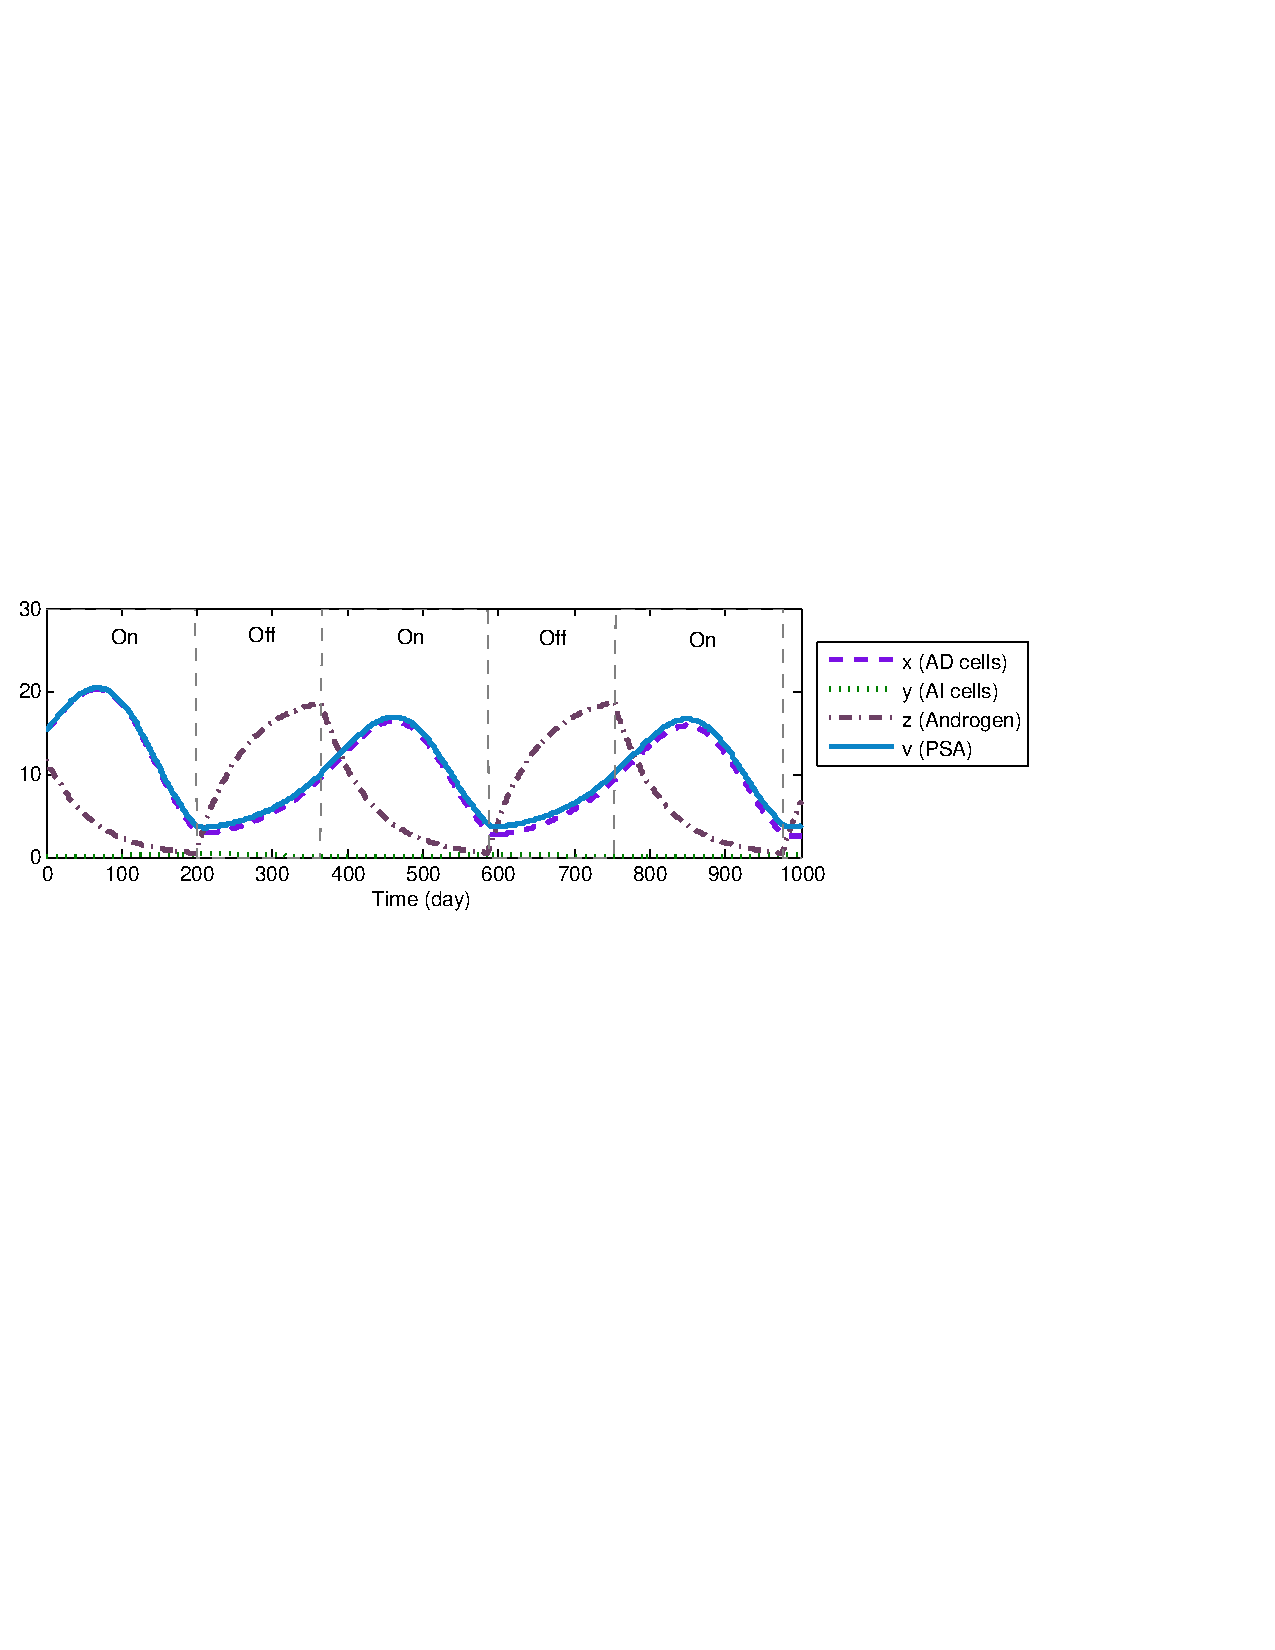
\includegraphics[scale=0.5]{fig-prostatetraj}
\caption{Simulated time profiles of $H_3$ model.}
\label{prostate-fig1}
 %\vspace{-0.7cm}
\end{figure}

\subsection{Personalized therapy design}
We next apply our parameter synthesis method to selecting suitable therapy and designing personalized treatment scheme for individual patients. Note that the parameter values in Table \ref{prostate} were estimated from clinical data of hundreds of patients \citep{bruchovsky07}. Among patients, the values of some parameters vary, which causes the variability in responsiveness to hormone therapy. We select a set of ``personalized parameters'' including $\alpha_y$ (the proliferation rate of AI cells), $\beta_y$ (the apoptosis rate of AI cells), $m_1$ (the mutation rate from AD to AI cells), and $z(0)$ (the initial androgen level). The values of these parameters can be either experimentally measured \citep{berges95} or computationally determined from PSA time serials data \citep{hirata10}.

Figure \ref{patients}(a-c) illustrates the PSA dynamics of $3$ patients with different personalized parameters under the same IAS treatment scheme ($r_0=4$, $r_1=10$). IAS prevents the relapse for Patient\#1 and delays the relapse for Patient\#2, but does not help Patient\#3. Figure \ref{patients}(d) shows that, by modifying the IAS scheduling parameters $r_0$ and $r_1$, the relapse of Patient\#3 can be avoided or delayed. Thus, we can formulate the personalized therapy design problem as a parameter synthesis procedure: (i) fill in parameter values of a patient to $H_3$; (ii) set the ranges of scheduling parameters as $r_0 \in [0,8)$ (nM) and $r_1 \in [8,15]$; (iii) check if $H_3$ can reach a state with $t=1000$ given the invariant $v \in [0,30]$ (i.e. no relapse). If the $\delta$-decision procedure returns $\mathsf{False}$, it means that androgen suppression therapy is not suitable for the patient. Otherwise, a treatment scheme containing feasible values of $r_0$ and $r_1$ will be returned, which could prevent or delay the relapse of the patient. Note that if $r_0=0$ is returned, it refers to the CAS scheme.

\begin{figure}[htb]
\centering
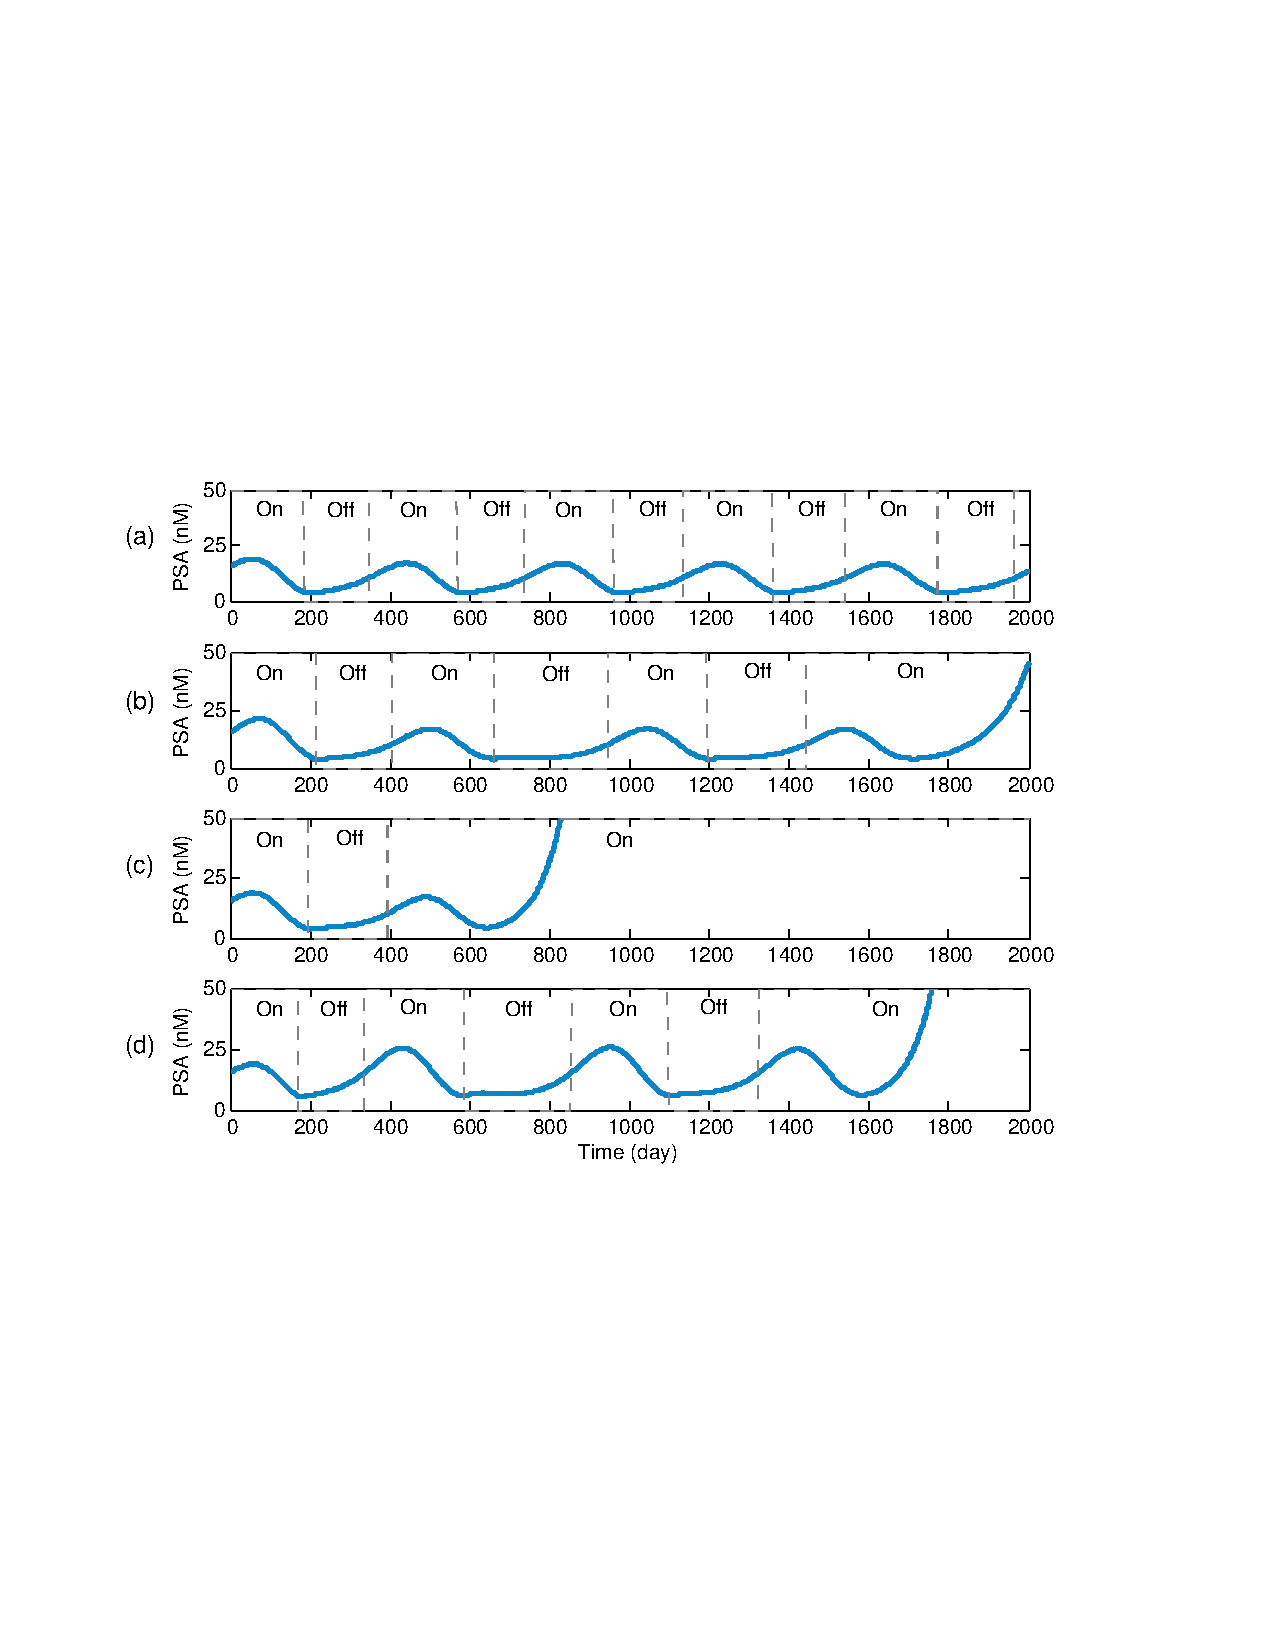
\includegraphics[scale=0.5]{fig-prostatetraj2}
\caption{Simulated PSA profiles of patients with different parameters. (a) Patient\#1: $\alpha_y=0.0242$, $\beta_y=0.0168$, $m_1=0.00005$, $z(0)=12$, $r_0=4$, $r_1=10$ (b) Patient\#2: $\alpha_y=0.24$, $\beta_y=0.13$, $z(0)=13$, $m_1=0.0001$, $r_0=4$, $r_1=10$ (c) Patient\#3: $\alpha_y=0.35$, $\beta_y=0.187$, $m_1=0.00005$, $z(0)=10$, $r_0=4$, $r_1=10$ (d) Patient\#3: $\alpha_y=0.035$, $\beta_y=0.187$, $m_1=0.00005$, $z(0)=10$, $r_0=6$, $r_1=15$.}
\label{patients}
 %\vspace{-0.7cm}
\end{figure}


We tested our method on real patients data collected by \cite{bruchovsky07}. The values of $\alpha_y$, $\beta_y$, $m_1$, and $z(0)$ for each selected patient were estimated by fitting the model to the PSA time serials data under the first $1.5$ cycles of IAS therapy (data available at http://www.nicholasbruchovsky.com/clinicalResearch.html). Table \ref{prostate2} summarized the suggested treatment scheme for selected patients. The in silico validation results are shown in Supplementary Materials.


\begin{table}[h]
\caption{Personalized hormone therapy scheme for selected patients\label{prostate2}}
\centering
\begin{tabular}{c|c|c|c|c|c}
\hline
Patient ID  & $\alpha_y$  & $\beta_y$ & $m_1$ & $z(0)$ & Suggested scheme  \\\hline
\#8 & 0.025 & 0.021  & 3.0E-5 & 8.23 & $r_0=5.0$, $r_1=11.2$ \\
\#10 & 0.019 & 0.009  & 5.9E-5 & 9.44 & $r_0=4.1$, $r_1=9.4$ \\
\#45 & 0.012  & 0.041  & 1.0E-5 & 12.61 & $r_0=3.8$, $r_1=12.2$ \\
\#97 & 0.031  & 0.015  & 2.3E-5 & 10.61 & $-$ \\
\hline
\end{tabular}
 %\vspace{-0.7cm}
\end{table}





